\newpage
\section{Descrizione architettura}
\subsection{Metodo e formalismo di specifica}

Per esporre l'architettura dell'applicazione si procederà con approccio top-down, partendo cioè da una visione generale delle componenti che distinguono il sistema, per poi analizzare in dettaglio la conformazione di tali componenti. 

Per descrivere in maniera formale l'architettura verranno impiegati lo standard UML 2.0 per i diagrammi dei package e delle classi e lo standard UML 2.4 per i diagrammi di attività e sequenza.

Laddove nella progettazione è stata necessaria l'introduzione di convenzioni per determinati elementi, queste verranno giustificate e presentate in dettaglio nella parte introduttiva della descrizione della componente stessa.


%La scelta di utilizzare Javascript come linguaggio su cui basare il progetto ha reso necessaria l'introduzione di alcune convenzioni per quanto riguarda i diagrammi UML utilizzati, in particolare quello dei package e delle classi.
%Poichè Javascript non implementa il costrutto class, tale formalismo verrà riferito ai moduli (che implementano il Module pattern di Javascript).

Viene fatto uso inoltre di un codice colori per distinguere la provvenienza dei moduli dell'applicazione. In particolare:

\begin{itemize}
\item verranno evidenziati in colore \textbf{giallo} i moduli da implementare;
\item in colore \textbf{verde} vengono proposti i moduli/librerie importati dal Core delle tecnologie utilizzate e da terze parti;
\item in colore \textbf{rosso} vengono evidenziati i moduli riutilizzati da MaaP.
\end{itemize}

\subsection{Conformazione generale dell'architettura}
L'architettura generale di MaaS si può dividere in 3 macrocomponenti:
\begin{itemize}
\item \textbf{Server REST} 
\item \textbf{Client} 
\item \textbf{Editor}
\end{itemize}

\begin{figure}[h]
\centering
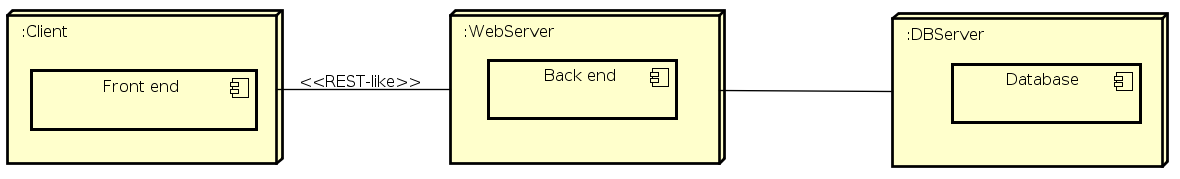
\includegraphics[width=0.8\textwidth]{res/sections/GeneralArchitecture.png}
\caption{Diagramma di deployment per l'architettura}
\end{figure}

L'architettura proposta segue il Design Pattern MVC. In particolare i ruoli di Model e Controller verranno implementati a livello di server, mentre il ruolo di View viene affidato al frontend.
L'intrefaccia tra le due componenti verrà gestita grazie ad un set di API disposto dal server REST: in questo modo si garantisce una totale indipendenza tra frontend e backend e concede a sviluppi futuri anche in altre piattaforme (ad esempio in app mobile) senza dover creare dei sistemi di integrazione ad-hoc.

Le tre macrocomponenti verranno descritte nel dettaglio in seguito su questo documento.

